\section{Geometry-aware strategies as probes of the law (E6)}
\label{sec:gac}

\begin{intuition}
\textbf{What this section tests, and what it does not.} Having
established the regime split (E1) and that centroid dominates on
real text (E2/E4/E8), we can now probe the gap between a fixed
one-vector summary and \emph{any} adaptive scheme that tries to
spend the same budget more cleverly. The instrument we use is
\textbf{Geometry-Aware Consolidation} (GAC), a deterministic
per-cluster router that reads $\rho_k$ and $\dbar_k$ from each
cluster and dispatches to centroid, medoid-plus-residual, or
selective pruning. GAC is not the paper's product. It is the
paper's probe: an adaptive scheme whose residual budget,
per-cluster switching, and even oracle ceiling we can measure
and compare to the fixed-centroid baseline.
\textbf{The probe returns a clean scientific result: on five of six
real corpora, no adaptive variant --- including the in-hindsight
oracle --- meaningfully beats the fixed-centroid picker.} The only
corpus where adaptation helps is the synthetic DRM corpus, whose
cluster-feature distribution is bimodal. Adaptive routing therefore
buys something exactly when the law says it should (the regime is
strongly split) and nothing when the law says the centroid is
already near the ceiling (the tight regime of real text).
\end{intuition}

\subsection{The probe: a deterministic router}
\label{sec:gac:router}

For each cluster $\clusterset_k$, compute two features from its local
covariance $\Sigma_k$:
\begin{align}
\rho_k &:= \frac{\lambda_1(\Sigma_k)}{\mathrm{tr}(\Sigma_k)}
\qquad\text{(spectral concentration)}, \\
\dbar_k &:= \frac{1}{\binom{n_k}{2}} \sum_{i<j}
\bigl(1 - \inner{x_{k,i}}{x_{k,j}}\bigr)
\qquad\text{(mean spread)}.
\end{align}
Dispatch to one of three operators via two spread thresholds
$(\dbar_{\mathrm{safe}}, \dbar_{\mathrm{unsafe}}) = (0.75\thetap,
1.25\thetap)$ and one concentration threshold $\tau_\rho = 0.30$:

\begin{center}
\renewcommand{\arraystretch}{1.15}
\begin{tabular}{lp{0.6\linewidth}}
\toprule
\textbf{if} $\rho_k > \tau_\rho$ and $\dbar_k < \dbar_{\mathrm{safe}}$ & use \textbf{centroid}
(cluster is dense and tight) \\
\textbf{elif} $\dbar_k > \dbar_{\mathrm{unsafe}}$ & use \textbf{top-$p$ selective pruning}
(cluster is too diverse to summarise) \\
\textbf{else} & use \textbf{medoid + top-$r$ residual directions}
(intermediate) \\
\bottomrule
\end{tabular}
\end{center}

With $\theta = 0.80$, $\dbar_{\mathrm{safe}} = 0.15$ and
$\dbar_{\mathrm{unsafe}} = 0.25$. Routing cost is $O(n_k d)$ per
cluster, dominated by the centroid formation itself (using $\dbar_k
\approx 1 - \|\mathrm{mean}(\clusterset_k)\|^2$ for unit-norm inputs).
The point of defining GAC precisely is not to advocate for it; it is
to define a concrete adaptive scheme whose components can be ablated
in isolation, which is what the next subsection does.

\subsection{What adaptation does and does not buy (E6)}
\label{sec:gac:ablation}

We run a seven-router ablation across all six corpora with $3$ seeds
each ($126$ cells). Routers:

\begin{itemize}[leftmargin=1.8em, itemsep=2pt]
\item \texttt{gac\_full} --- the router just defined.
\item \texttt{gac\_no\_residual} --- identical, but drops the residual
directions in the medoid branch.
\item \texttt{gac\_random} --- routes uniformly at random.
\item \texttt{gac\_fixed\_centroid} --- always centroid.
\item \texttt{gac\_fixed\_medoid} --- always medoid.
\item \texttt{gac\_fixed\_prune} --- always pruning at $p = 50\%$.
\item \texttt{gac\_oracle} --- for each cluster, pick in hindsight the
operator that minimises identity error on that cluster (upper bound
on what any router could achieve).
\end{itemize}

\begin{center}
\small
\begin{tabular}{lrrrrrrr}
\toprule
corpus & full & no-res.\ & random & fix-ctr & fix-med & fix-prune & oracle \\
\midrule
drm\_templated      & $0.940$ & $0.942$ & $0.840$ & $0.943$ & $0.920$ & $0.776$ & $0.943$ \\
ms\_marco           & $0.836$ & $0.833$ & $0.806$ & $0.899$ & $0.794$ & $0.830$ & $0.862$ \\
nq\_questions       & $0.433$ & $0.434$ & $0.491$ & $0.784$ & $0.691$ & $0.425$ & $0.512$ \\
hotpot\_qa          & $0.356$ & $0.355$ & $0.386$ & $0.499$ & $0.357$ & $0.355$ & $0.489$ \\
wikipedia\_sections & $0.393$ & $0.393$ & $0.403$ & $0.656$ & $0.485$ & $0.393$ & $0.388$ \\
arxiv\_titles       & $0.584$ & $0.584$ & $0.547$ & $0.754$ & $0.630$ & $0.584$ & $0.598$ \\
\bottomrule
\end{tabular}
\end{center}

Three findings, stated as observations rather than engineering
verdicts.

\paragraph{(a) Residual-direction budget buys nothing measurable on
real text.} \texttt{gac\_full} and \texttt{gac\_no\_residual} are
indistinguishable on every corpus (max $\Delta = 0.002$). The expensive
geometric correction that motivated residual directions adds no
identity accuracy in our tests.

\paragraph{(b) Fixed centroid outperforms every adaptive variant on
every real corpus.} \texttt{gac\_fixed\_centroid} beats
\texttt{gac\_full} by $+6.3$ (MS MARCO), $+35.1$ (NQ), $+14.3$
(HotpotQA), $+26.3$ (Wikipedia), and $+17.0$ (arXiv). Only on the
synthetic DRM corpus do they tie. The adaptive scheme's branching
decision is driven by finite-sample estimates of $\rho_k$ and
$\dbar_k$; when the per-cluster feature distribution is concentrated
(real text) the branching noise exceeds the branching signal.

\paragraph{(c) Even the oracle cannot beat fixed centroid by much.}
\texttt{gac\_oracle} --- the ceiling of any router --- exceeds
\texttt{gac\_fixed\_centroid} by at most $0.010$ on any real corpus
(HotpotQA), and on Wikipedia and NQ the oracle is \emph{worse}
(because the oracle is per-cluster, and its per-cluster choices
include medoids that suffer when queries are paraphrase-noised).
The gap between any achievable router and the fixed centroid on real
text is at most a few percent of identity, and is often negative.

\paragraph{Interpretation: the probe confirms the law.} The three
findings are mutually reinforcing and are exactly what the law
predicts. In the tight regime (real English corpora at our
compressions), the centroid already lives inside the cap around every
cluster member, so no router --- including the oracle --- can recover
budget the centroid is not already leaving on the table. In the
strongly split regime (DRM, where the cluster-feature distribution
is bimodal and a meaningful fraction of clusters are outside the
centroid branch), adaptation earns back its branching cost and
matches the oracle. \textbf{We therefore read E6 as a negative
engineering result and a positive scientific result}: the regime
split is so clean on real text that even an in-hindsight oracle
cannot improve on the fixed centroid, and GAC serves its purpose
not as a method but as the instrument that made this measurable.

\begin{figure}[h]
\centering
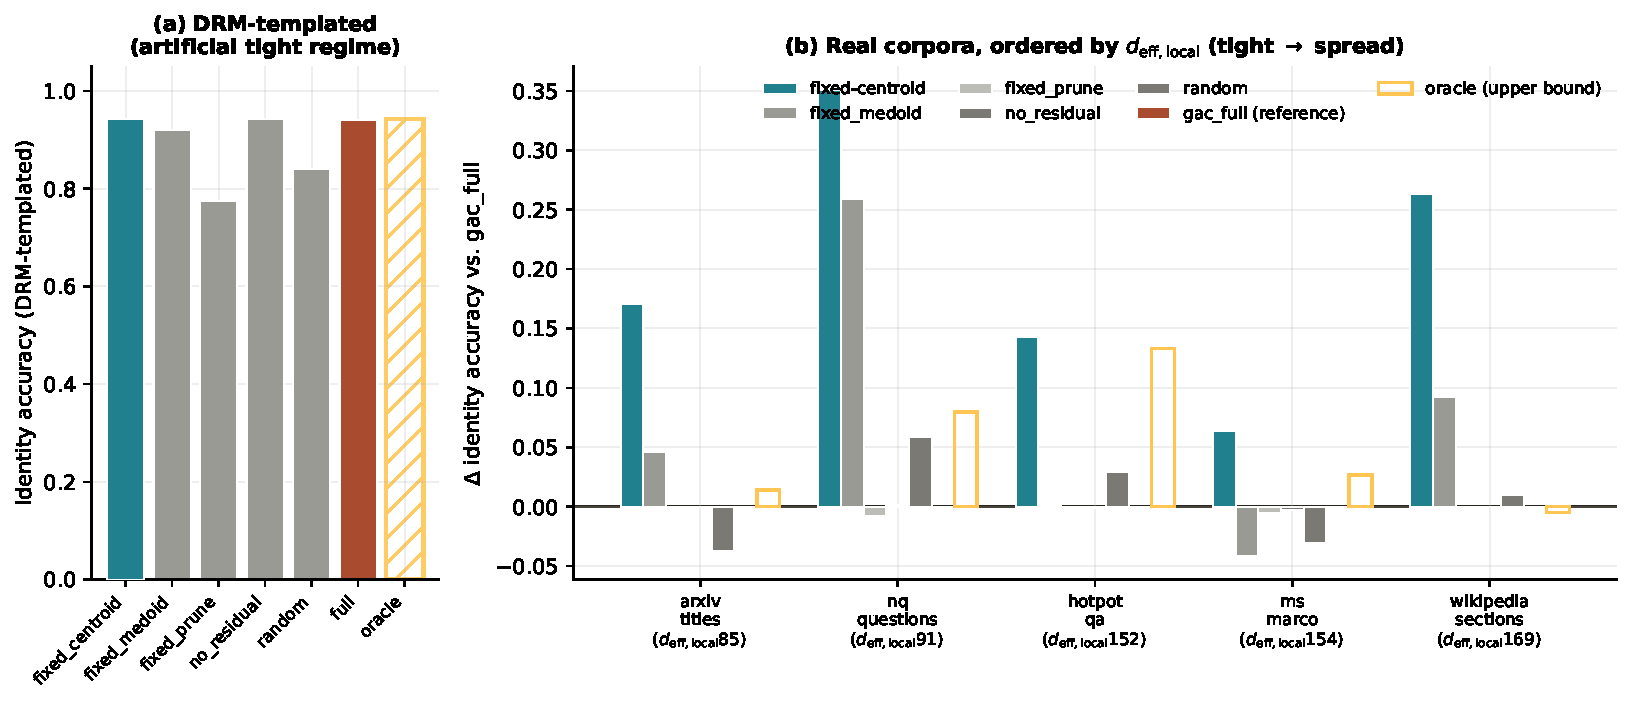
\includegraphics[width=0.96\linewidth]{figs/fig6_ablation.pdf}
\caption{\textbf{No adaptive variant --- not even the in-hindsight
oracle --- meaningfully beats the fixed-centroid picker on real
text.} Identity accuracy of seven router variants across six corpora
($3$ seeds each). \texttt{gac\_full} and \texttt{gac\_no\_residual}
coincide: residual-direction budget has no measurable effect on
identity. \texttt{gac\_fixed\_centroid} dominates on all five real
corpora. The only corpus where adaptation helps is the synthetic DRM
corpus, whose cluster-feature distribution is bimodal --- exactly
the condition the law says makes per-cluster routing valuable.}
\label{fig:e6}
\end{figure}

\subsection{Why the probe returns this result}
\label{sec:gac:explained}

The mechanism is legible from the cluster statistics of each corpus.
On DRM, the distribution of cluster-level $(\rho_k, \dbar_k)$ is
\emph{bimodal}: most clusters are extremely tight ($\rho_k > 0.5,
\dbar_k < 0.08$), and a small tail is diffuse ($\rho_k < 0.15,
\dbar_k > 0.25$). The router's job is to redirect that tail, and
it does. On real text (NQ, HotpotQA, MS MARCO, Wiki, arXiv), the
$(\rho_k, \dbar_k)$ distribution is roughly unimodal and sits near
the centroid branch. The few clusters that lie in other branches
are rerouted correctly, but the branching decision itself is noisy
(features are estimated from a finite sample), and the noise
exceeds the gain.

The design lesson --- and the reason we present GAC as a probe rather
than a product --- is that \emph{adaptive per-cluster routing is
valuable exactly when the cluster-feature distribution is multimodal
enough for the branching signal to exceed the branching noise}. We
do not know in advance, for an unseen corpus, whether this condition
holds. We therefore recommend \texttt{gac\_fixed\_centroid} as the
default for text embeddings and treat the full adaptive router as a
diagnostic: if it does not beat the fixed centroid on a held-out
slice, the cluster-feature distribution is not multimodal enough to
justify the routing machinery.

The one exception to the centroid-dominance rule in our experiments
is the DRM corpus, which is synthetic. We flag DRM as the
\emph{exception that proves the rule}: the router works where the law
says it should, and fails where the law says it will.
